\subsection{Spectral Clustering}
We tested 18 different configurations of the Spectral Clustering algorithm on each dataset, using three different eigen 
solvers (`lobpcg', `amg', and `arpack') with two different \texttt{assign\_labels} parameters (`kmeans' and `cluster\_qr') 
and three different values for \texttt{n\_neighbors}, depending on the dataset. The selected values for this last hyperparameter
 are presented in Table \ref{tab:hyper-choices-spectral}. For each configuration, we ran the algorithm 10 times and saved the 
 results independently to analyze the evolution of the metrics rather than merely obtaining the value that minimizes the k-means 
 cost function. This approach differs from using the pre-implemented hyperparameter \texttt{n\_init} in sklearn, which focuses 
 solely on minimizing the cost function.

\subsubsection{Hyperparameter Study}

The values selected for the hyperparameters shown in Table \ref{tab:hyper-choices-spectral} were appropriate for each dataset. 
In the case of the Hepatitis dataset, smaller values for \texttt{n\_neighbors} were required primarily due to two factors: the 
limited size of the dataset and the significant imbalance between the two classes (one class was much smaller than the other). 
Using a smaller value for this hyperparameter helped capture local relationships between points, emphasizing the structure of 
small, tightly-knit groups or clusters within the data. In contrast, for the other two datasets (Mushroom and Pen-based),
 larger values were necessary to maintain the connectivity of the graph.



 Regarding the tolerance, for Hepatitis and Mushroom, the value used was the default one, 0.0, which means that the tolerance 
 for convergence is the default value of each of the eigen solvers. However, for the Pen-based dataset, a tolerance of 
 \( 1 \times 10^{-3} \) was used, as some issues related to convergence were encountered.


\begin{table}[h!]
    \centering
    \begin{tabular}{|c|c|c|c|}
    \hline
    \textbf{Hyperparameter}     & \textbf{Hepatitis} & \textbf{Mushroom} & \textbf{Pen-based} \\ \hline
    \texttt{n\_clusters}        &  2      &   2    &  10         \\ \hline
    \texttt{n\_neighbors}       &  [5, 7, 10]  &   [100, 150, 200]  &  [150, 200, 250]   \\ \hline
	\texttt{eigen\_tol}        &  0.0     &   0.0    &  1e-3    \\ \hline
    \end{tabular}
	\caption{Hyperparameters chosen for each dataset.}\label{tab:hyper-choices-spectral}
    \end{table}



\subsubsection{Best runs}


For each of the datasets, we extracted the run that achieved the best score for each of the metrics, which can be found in 
Table \ref{tab:spectral_best_runs_spectral_hep-m} and \ref{tab:spectral_best_runs_spectral_pb}. As in the case of OPTICS, 
some metrics, such as ARI and NMI, seem to perform much better on the Pen-based dataset than on Hepatitis. The label
 assignment method was k-means, while for the eigen solver, lobpcg appeared frequently in Hepatitis and Mushroom, and `arpack' 
 and `amg' were more suitable for the Pen-based dataset.



 The best run, obtained according to the NMI metric, was plotted after applying the dimensionality reduction technique that 
 showed a better clustering split. It reflected the numerical value of the metric, as the classification was better for the 
 Pen-based dataset than for Mushroom, and also better for Mushroom than for Hepatitis. Nevertheless, the graphical representation
  could reveal inner structures of the data that are not directly related to the classes of the dataset. The result can be found
   in Figure \ref{fig:spectral-clusters-br-pca}.

\begin{table}[h!]
	\centering
	\begin{tabular}{|c|c|c|c|c|c|c|c|c|c|c|c|}
		\hline
		& \multicolumn{4}{c|}{\textbf{Hepatitis}} & \multicolumn{4}{c|}{\textbf{Mushroom}} \\ \hline
		\textbf{Metric} &  \textit{eigen solver} & \textit{n} & \textit{assign label} & \textit{Value}  &\textit{eigen solver} & \textit{n} & \textit{assign label} & \textit{Value} \\ \hline
		ARI            & lobpcg       & 10   & kmeans & 0.0499 & lobpcg   & 100  & kmeans & 0.1912  \\ \hline
		NMI            & lobpcg        & 7    & cluster\_qr& 0.1400&  lobpcg    & 100  & kmeans & 0.2374 \\ \hline
		DBI            & lobpcg    & 5 &kmeans & 1.4384   & lobpcg   & 100 & kmeans & 1.1623 \\ \hline
		Silhouette     & lobpcg   & 10 &kmeans &  0.1749  & lobpcg  & 100 & kmeans & 0.2819 \\ \hline
		CHS            & lobpcg    & 10 &kmeans & 35   & lobpcg  & 100 & kmeans & 2940 \\ \hline
	\end{tabular}
	\caption{Best configurations and their corresponding parameter values (\textit{eigen solver} for \texttt{eigen\_solver}, \textit{n} for \texttt{n\_neighbors} and \textit{assign label} for \texttt{assign\_label}) and the metric values across the Hepatitis and Mushroom datasets.}
	\label{tab:spectral_best_runs_spectral_hep-m}
\end{table}

\begin{table}[h!]
	\centering
	\begin{tabular}{|c|c|c|c|c|}
		\hline
		&  \multicolumn{4}{c|}{\textbf{Pen-Based}} \\ \hline
		\textbf{Metric}  &\textit{eigen solver} & \textit{n} & \textit{assign\_label} & \textit{Value} \\ \hline
		ARI             & arpack  & 150 & kmeans & 0.6899 \\ \hline
		NMI            & arpack   & 150 & kmeans & 0.7811 \\ \hline
		DBI            & amg & 250 & kmeans & 1.3044 \\ \hline
		Silhouette      & amg & 250 & cluster\_qr & 0.2920\\ \hline
		CHS            & amg & 250 & cluster\_qr & 2640\\ \hline
	\end{tabular}
	\caption{Best configurations according to the metrics values, and their corresponding hyperparameters (\textit{eigen solver} for \texttt{eigen\_solver}, \textit{n} for \texttt{n\_neighbors} and \textit{assign label} for \texttt{assign\_label}) for the Pen-based dataset.}
	\label{tab:spectral_best_runs_spectral_pb}
\end{table}



\begin{figure}[H]
	\centering
	\begin{subfigure}{0.32\textwidth}
		\centering
		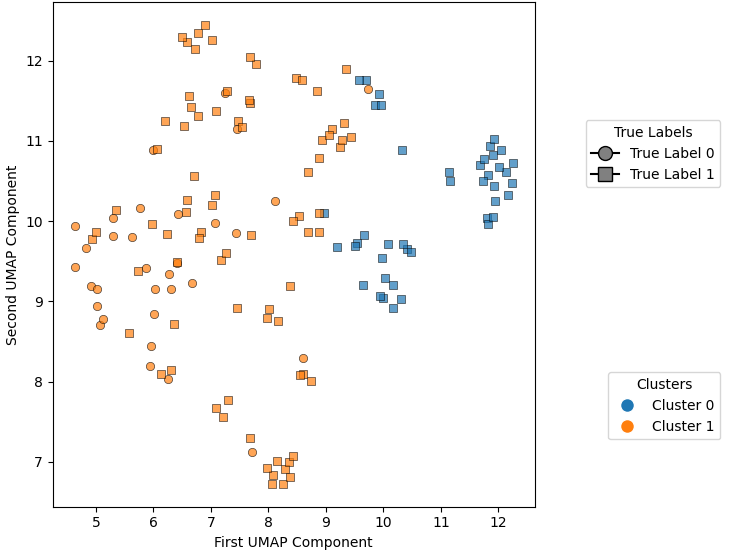
\includegraphics[width=0.7\linewidth]{figures/Spectral/hepatitis/best_run_NMI_umap.png}
		\caption{Hepatitis Dataset (UMAP) \\ (\texttt{n\_neighbors = 7}, \\  \texttt{eigen\_solver = lobpcg}, \\ \texttt{assign\_labels = cluster\_qr})}
	\end{subfigure}
	\hfill
	\begin{subfigure}{0.32\textwidth}
		\centering
		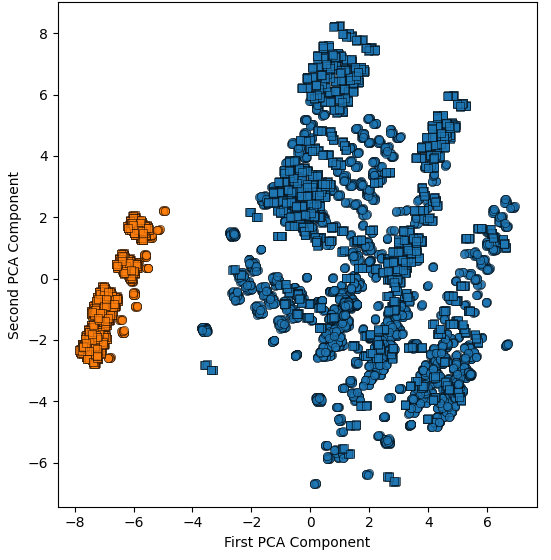
\includegraphics[width=0.7\linewidth]{figures/Spectral/mushroom/best_run_NMI_pca.png}
		\caption{Mushroom Dataset (PCA) \\ (\texttt{n\_neighbors = 100}, \\  \texttt{eigen\_solver = lobpcg}, \\ \texttt{assign\_labels = kmeans})}
	\end{subfigure}
	\hfill
	\begin{subfigure}{0.32\textwidth}
		\centering
		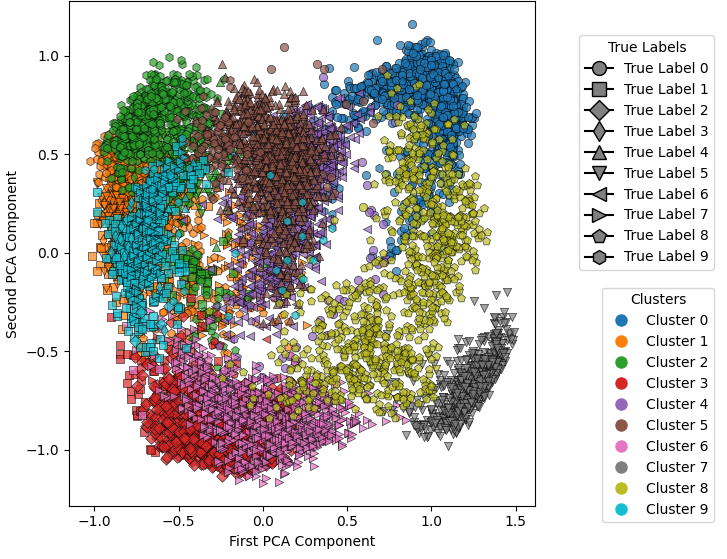
\includegraphics[width=0.7\linewidth]{figures/Spectral/pen-based/best_run_NMI_pca.png}
		\caption{Pen-Based Dataset (PCA) \\ (\texttt{n\_neighbors = 150}, \\  \texttt{eigen\_solver = arpack}, \\ \texttt{assign\_labels = kmeans})}
	\end{subfigure}
	\caption{Visualization of the resulting clusters for each dataset, with the best configurations, according to the metric NMI 
	in Table \ref{tab:spectral_best_runs_spectral_hep-m} and \ref{tab:spectral_best_runs_spectral_pb}.}
	\label{fig:spectral-clusters-br-pca}
\end{figure}

